\section{Description technique}

Comme cité précédemment, notre application a été codé à l'aide de la librairie JavaFX. Ainsi, toute notre implémentation technique est basée sur cette dernière. JavaFX utilise des fichiers FXML pour séparer la logique de la vue TODO TODO TODO

\subsection{Serialisation}
En Java, la sérialisation s'effectue à l'aide de l'interface \og Serializable \fg{}. Par conséquent, chaque classes de Java implémentant cette dernière telle que \og String \fg{}, peut être sérialiser et désérialiser à volonté. Cependant, la majorité des classes JavaFX n'implémente pas cette interface. En effet, les objets JavaFX s'utilisent de façon dynamiques et interagissent entre eux. 

Pour combler ce manque, nous devons nous même implémenter la sérialisation des classes JavaFX que nous sommes susceptible d'utiliser.

\begin{figure}[h]
    \caption{Diagramme de la sérialisation simplifié}
    \centering
    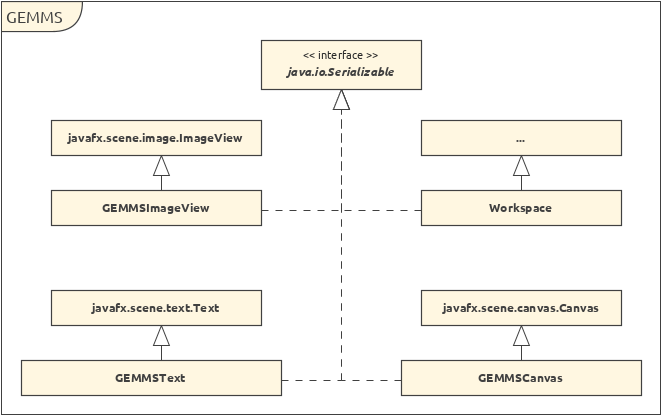
\includegraphics[scale=0.6]{serialisation_diagram.png}
    \label{fig:seri_diag}
\end{figure}

Sur la figure \ref{fig:seri_diag}, nous pouvons voir un diagramme simplifié de l'implémentation de la sérialisation. Dans notre application, nous allons utilisé les classes de base suivantes : ImageView, Text et Canvas. Nous devons donc spécialiser ces classes afin qu'elles puissent implémenter l'interface \og Serializable \fg{}. 

Étant donné que les classes JavaFX possèdent énormément de fonctionnalités, sérialiser l'entier de celles-ci nous demanderait beaucoup trop de temps. C'est pourquoi nous nous contentons uniquement des paramètres utilisés tel que la largeur, la hauteur, la position, etc. 

TODOTDOTDO TDO




